\chapter{Systementwurf}

\section{Symbolverzeichnis}


\begin{table}[htbp]
    \centering
    \begin{tabular}{l l}
        \hline
        \textbf{Symbol/Formelzeichen} & \textbf{Beschreibung} \\
        \hline
        \((KS)_E\) & Ursprung des Koordinatensystems auf der schiefen Ebene \\
        \( _{(E)}\vec{p}(t) \) & 3D-Vektor der Gesamtbewegung in Ebene \((KS)_E\)\\
        \(_{(E)}\vec{p_B} (t) \) & 3D-Vektor der reinen Bewegung in Ebene \((KS)_E\) \\
        \(_{(E)}\vec{p_0}\) & 3D-Startvektor. Durch Eingabe des Nutzers (Spaltbreite)\\
        \(z(t)\) & Bewegungsgleichung der Robotertrajektorie \\
        \(\hat{z}\) & Eingabe des Benutzers für die Hubhöhe\\
        \(\omega\) & Kreisfrequenz \\
        \(f\) & Eingabe des Nutzers für die Frequenz \\
        \(W\) & Physikalische Arbeit \\
        \(F\) & Physikalische Kraft \\
        \(P\) & Physikalische Leistung \\
        

        \hline
    \end{tabular}
    \caption{Symbol- und Formelzeichenverzeichnis}
\end{table}

\section{Bewegungsprofil des Paddel-Mischers}

\begin{figure}[h]
    \centering
    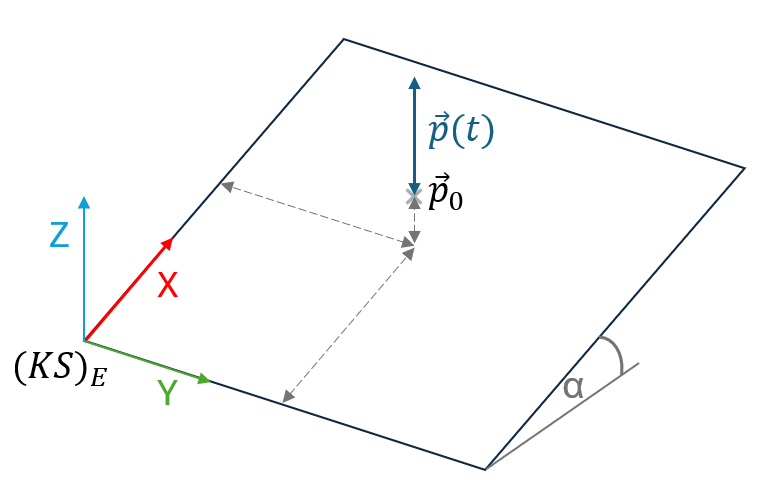
\includegraphics[width=0.8\textwidth]{bilder/KS_E-Koordinatensystem_Ebene.png}
    \caption[Visualisierung des Koordinatensystems auf der schiefen Ebene]{Visualisierung des Koordinatensystems auf der schiefen Ebene (eigene Darstellung)}\label{fig:VisualisierungKoordinatensystemSchiefe}
\end{figure}

\noindent Im Folgenden werden die drei Parameter zur reproduzierbaren Beschreibung der Paddel Bewegung in allen drei Bewegungsrichtungen beschrieben. Hierbei ist \( _{(E)}\vec{p}(t) \) stellvertretend für die Gesamtbewegung in Koordinatensystem \((KS)_E\). \(_{(E)}\vec{p_B} (t) \) beschreibt die veränderliche Position ausgehend von \(_{(E)}\vec{p_0}\).\\

\textbf{Allgemein:}


\begin{equation}
    \begin{aligned}
        _{(E)}\vec{p}(t) &= _{(E)}\vec{p_B}(t) + _{(E)}\vec{p_0}\\
        \text{mit}\\
        _{(E)}\vec{p}_B(t) &= _{(E)}\left(x_B(t), y_B(t), z_B(t)\right)\\
        _{(E)}\vec{p_0} &= _{(E)}\left(x_0, y_0, z_0\right)
    \end{aligned}
    \label{eq:generelleBewegung}
\end{equation}

\autoref{eq:generelleBewegung} ist unabhängig von der eingeleiteten Bewegungsform und Richtung. Es können in \(\vec{p}_B(t)\) alle möglichen Bewegungsformen dargestellt werden.\\

Hier folgt nun die Errechnung anhand einer sinus-förmigen Bewegung entlang der Z-Achse:

\begin{equation}
    \begin{aligned}
        _{(E)}\vec{p}_{0} &= (x_{0}, y_{0}, z_{0})\\
        _{(E)}\vec{p}(t) &= (x, y, z(t)) + \vec{p}_{0}  
    \end{aligned} 
\end{equation}

\( z(t) \) ist definiert durch:

\begin{equation}
    z(t) = -\hat{z}(\cos(\omega t)-1)  \quad \text{mit} \quad \hat{z} = \frac{h}{2}
\end{equation}

und \( \omega = 2 \pi f = \frac{2 \pi}{T} \).

Zum Beispiel, bei \( t = 0 \):

\begin{equation}
    z(0) = -\hat{z}(1-1) = 0
\end{equation}

Beispiel bei \( t = \frac{1}{4}T \):

\begin{equation}
    \begin{aligned}
        z\left(\frac{1}{4}T\right) &= -\hat{z}\left(\cos\left(\frac{2\pi T}{T \cdot 4}\right) - 1\right) \\
        &= -\hat{z}\left(\cos\left(\frac{\pi}{2}\right) - 1\right) \\
        &= -\hat{z}(0 - 1) = \hat{z} = \frac{1}{2} h
    \end{aligned}
\end{equation}

Und bei \( t = \frac{1}{2}T \):

\begin{equation}
    \begin{aligned}
        z\left(\frac{1}{2}T\right) &= -\hat{z}\left(\cos\left(\frac{2\pi T}{T \cdot 2}\right) - 1\right) \\
        &= -\hat{z}\left(\cos(\pi) - 1\right) \\
        &= -\hat{z}(-1 - 1) = 2\hat{z} = h
    \end{aligned}
\end{equation}


wobei \( _{(E)}\vec{p(t)} \) die Bewegung des Paddel-Mittelpunkts und \( _{(E)}\vec{p}_{0} \) den Mittelpunkt auf dem Einwegbeutel repräsentiert.

\begin{figure}[h]
    \centering
    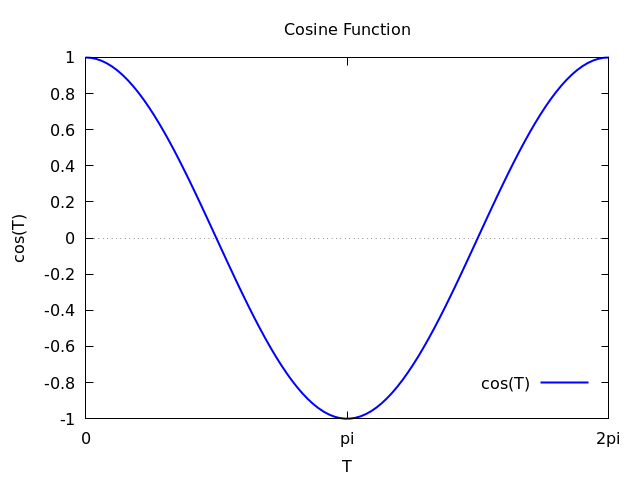
\includegraphics[width=0.8\textwidth]{bilder/cosine-plot.png}
    \caption[Kosinusfunktion]{Klassische Kosinusfunktion (\( cos(t) \)) (eigene Darstellung)}\label{fig:Kosinusfunktion}
\end{figure}
\FloatBarrier

\begin{figure}[h]
    \centering
    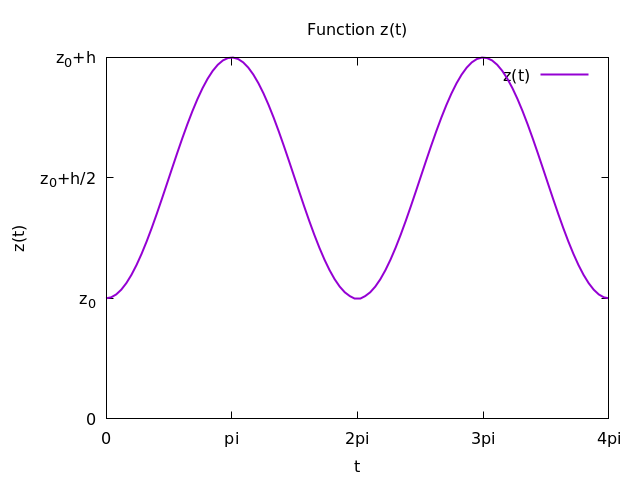
\includegraphics[width=0.8\textwidth]{bilder/cosine-plot_real.png}
    \caption[Darstellung der Paddelbewegung anhand der Cosinusfunktion]{Darstellung der Paddelbewegung in Z-Richtung anhand der Cosinusfunktion \( z(t) = -\hat{z}(\cos(\omega t)-1) \) (eigene Darstellung)}\label{fig:PaddelbewegungCos}
\end{figure}
\FloatBarrier



Beispiel Sinus-Bewegung in \( _{(E)}\) Z-Richtung:
\begin{equation}
    \begin{aligned}
        x &= x_B + x_0\\
        y &= y_B + y_0\\
        z(t) &= \hat{z}\left( 1 - \cos(\omega t) \right) +z_0\\
        \text{mit}\\
        &\hat{z} = 2h\\
        &\omega = 2\pi f
    \end{aligned}
\end{equation}

\section{Definition der Leistungseinbringung für den Mischprozess}

Allgemein gilt:

\begin{equation}
    W = \int_{t_1}^{t_2} \vec{F}(\vec{s(t)})\cdot d \vec{s}
\end{equation}

\noindent Wenn die Kraftrichtung der Bewegungsrichtung gleicht und beide Vektoren in dieselbe Richtung zeigen gilt:

\begin{equation}
    W = F \cdot s \text{   und   } P = \frac{W}{dt}
\end{equation}

\noindent In unserem Fall zeigt die Kraft \(F_z\) in die Bewegungsrichtung \(z\), aber sie ist nicht konstant. Daher gilt:

\begin{equation}
    \begin{aligned}
        W = \int_{t_1}^{t_2} F_z (z(t))\cdot dz\\
        W = \int_{t_1}^{t_2} F_z (t)\cdot dz
    \end{aligned}
\end{equation}

Der Zusammenhang von Kraft und Weg ist in \autoref{fig:EingebrachteLeistungWegZeit} dargestellt. Bei \(z_0\) liegt die maximale Kraft an, da der Abstand zum Einwegbeutel am geringsten ist.

\begin{figure}[h]
    \centering
    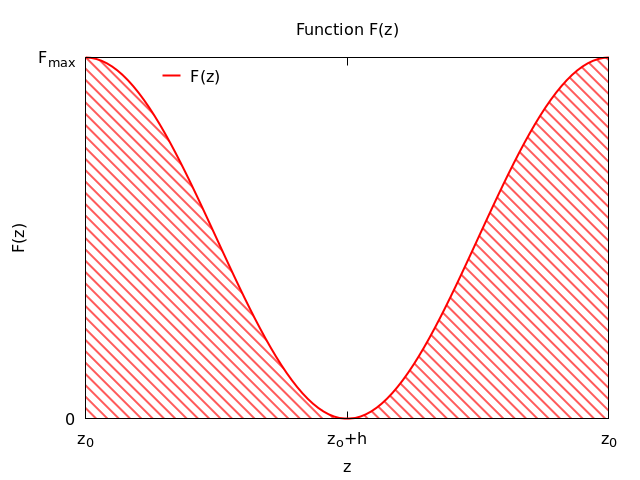
\includegraphics[width=0.8\textwidth]{bilder/force-over-distance.png}
    \caption[Eingebrachte Leistung Weg-über-Zeit-Diagramm]{Eingebrachte Leistung Weg-über-Zeit-Diagramm (eigene Darstellung)}\label{fig:EingebrachteLeistungWegZeit}
\end{figure}
\FloatBarrier

\textbf{Diskrete Messpunkte:}
\begin{equation}
    W = \sum_{t \in \{t_0; t_0 + T; T_0 + 2T; \dots; t_n\}}^{} F_z(t) \cdot \Delta z(t) = \sum_{t \in \{t_0; t_1; \dots; t_n\}}^{} F_z (t) \cdot (z(t+1)-z(t))
\end{equation}